%!TEX root = ../memoire.tex

\chapter{Implémentation et évaluation du système}\label{eval}

Au chapitre précédent, nous avions extraits des informations précieuses de VerbNet à l'aide de scripts Python. Nous avons ainsi fait usage de ces informations en les implémentant dans GenDR. Ce chapitre est séparé en trois parties. D'abord nous expliquons comment les dictionnaires fonctionnent après l'implémentation et comment ils communiquent entre eux. Puis, nous allons reconstruire la réalisation d'un arbre syntaxique de surface en expliquant comment les dictionnaires et règles de grammaires intéragissent dans cette nouvelle version de GenDR. Puis finalement, nous traiterons de l'évaluation du système et les modifications nécessaires pour un meilleur rendement.

\section{Implémentation des verbes et de leurs patrons de régime: lexicon.dict et gpcon.dict}

Au chapitre \ref{chapgendr}, nous avions démontré comment l'information lexicale s'encodait dans GenDR. Nous avions deux dictionnaires: un dictionnaire de sémantème et un dictionnaire de lexème. À la suite des informations extraites sur les patrons de régime, nous avons maintenant un troisième dictionnaire: un dictionnaire de patron de régime. L'implémentation de cette ressource a engendré un ajustement du lexicon pour tenir compte de la nouvelle architecture qui règne dorénavant entre elle et le dictionnaire de gp.

\subsection{Lexicon.dict 2.0}
Comme nous l'avons vu à la section \ref{dictio}, GenDR traitait les verbes et leurs comportements syntaxiques directement dans le lexicon. Dorénavant, le lexicon est séparé en diverses sections. La première section \texttt{DEFAULT ATTRIBUTES} décrit les classes générales de GenDR. Elle contient les verbes, les noms, les adjectifs, les adverbes, les prépositions et les classes que nous avons vu précédemment qui traite les lexèmes qu'on ne veut pas encoder dans le dictionnaire: montant, date, lieu, noms propres, acronymes,etc. Les grandes classes possèdent très peu d'information syntaxique, car dorénavant cela va dans le gpcon. Elles contiennent néanmoins des informations très importantes. Notamment, la partie du discours, des traits morpho-syntaxiques et l'identifiant du patron de régime à utiliser par la classe. Seuls les verbes n'ont pas d'identifiant de patrons de régime dans cette section, puisqu'il s'agit de la classe de lexèmes qui a les patrons de régime les plus irréguliers. Ceux-ci sont encodés dans les classes verbales de VerbNet que nous avons extrait. En ce qui concerne les autres classes, nous leurs avons imposé un patron de régime par défaut qui permet pour l'instant de réaliser une grande quantité de construction syntaxiques. Vous pouvez en constater un exemple dans la figure~\ref{classedef} sous la classe \texttt{NOUNS}.

\begin{lstlisting}[language=XML, caption = Attributs par défaut des classes, label=classedef]
/*
=======================================================
                  DEFAULT ATTRIBUTES
=======================================================
*/

// ================= VERBS =================

// VERB
// ----

verb {
  dpos = V
  spos = verb
}

// ================= NOUNS =================

// NOUN
// ----
// Common nouns.

noun {
  dpos = N
  spos = noun
  countable = yes
  gp = { id=NP dia=1}
}
\end{lstlisting}

La prochaine section \texttt{VERBNET MEMBERS} contient les membres des classes verbales de VerbNet que nous avions extrait avec le script Python (voir figure \ref{scriptmember}). Sont listés tous les 6393 verbes ainsi que la classe de VerbNet (ou la sous-classe) qui leur correspond. C'est aussi dans cette section que la désambiguisation des verbes est explicitée. Tel que nous l'avons démontré à la section précédente, nous avions extraits les membres de classes de VerbNet, puis nous avons désambiuiser les formes identiques puisque certains verbes ont la même forme, mais des sens différents. Cette partie de la section en montre un exemple. On a désambiguiser la forme \lex{order} en répertoriant qu'elle apparaissait à deux reprises dans le corpus de VerbNet. Dans le premier cas elle pointait vers la classe \texttt{get-13.5.1} et il s'agit du sens \sem{passer une commande} tandis que le deuxième signfie \sem{donner un ordre} \texttt{order-60-1}.

\begin{lstlisting}[language=XML, caption = Partie membre du lexicon]
/*
 =======================================================
                      VERBNET MEMBERS
 =======================================================
*/
"open up" : "establish-55.5-1"
operate : "other_cos-45.4"
oppose : "amalgamate-22.2-3"
ordain : "appoint-29.1"
order_1 : "get-13.5.1"
order_2 : "order-60-1"
organize_1 : "create-26.4"
organize_2 : "establish-55.5-1"
organize_3 : "force-59-1"
originate : "establish-55.5-1"
ornament_1 : "butter-9.9"
ornament_2 : "fill-9.8"
ornament_3 : "illustrate-25.3"
\end{lstlisting}

La troisième section est \texttt{VERBNET CLASSES}. Cette section décrit les diverses classes de VerbNet en deux traits. D'abord, la diathèse est décrite différement que dans GenDR 1.0 . Ce trait décrit la correspondance des actants sémantiques et syntaxiques en précisant l'ordre. Par exemple, une diathèse où le premier actant sémantique est le premier actant syntaxique, mais le troisième actant sémantique est le deuxième actant syntaxique sera représentée ainsi:  dia=132 (ça implique I:1 II:3 III:2). Ces informations permettront à GenDR de faire la correspondance des actants entre la RSem et la RSyntP. Les informations contenues (restrictions, etc.) dans les actants syntaxiques sont encodées dans le dictionnaire de patron de régime. Puis finalement, chaque classe verbale est dotée d'un trait \texttt{id} qui dicte au système quel patron de régime utiliser pour cette classe verbale en fonction de la diathèse imposée.

Finalement, c'est par l'entremise des trois sections que nous venons de vous présenter que nous avons implémenté l'architecture de VerbNet dans notre système. Le mécanisme d'héritage des traits que nous avions exposé à la section \ref{dictio} est réutilisé autrement. Les membres pointe vers les classes ou les sous-classes de VerbNet. Les sous-classes pointent vers les classes qui les domine, et les classes non-dominées pointe vers la classe 'verb' qui contient les attributs par défaut des verbes. Ce mécanisme d'héritage devrait pouvoir transmettre les paires de patrons de régime et de diathèse ainsi que les attributs par défaut. Si le système fonctionne bien, le mécanisme d'héritage nous permet de désaturer le dictionnaire et de calquer l'architecture de VerbNet correctement. Donc, les identifiants des gp ont une entrée dans le gpcon. C'est là qu'on décrit explicitement les comportements syntaxiques régis par un gp donné.

\begin{lstlisting}[language=XML, caption = Partie: Classes de VerbNet]
/*
=======================================================
                   VERBNET CLASSES
=======================================================
*/

"tell-37.2": verb {
  gp = { id=NP_V_NP  
	       dia=12 } // John informed me.
  gp = { id=NP_V_NP_PP_of_topic  
	       dia=123 } // John informed me of the situation. }
"tell-37.2-1": "tell-37.2" {
  gp = { id=NP_V_NP  
	       dia=12 } // Ellen told a story.
  gp = { id=NP_V_NP_PP_to_recipient 
		     dia=123 } // Ellen told a story to Helen.
  gp = { id=NP_V_NP_Dative_NP   
	       dia=132 } // Ellen told Helen a story. Ellen told me, 'Leave the room.'
  gp = { id=NP_V_NP
		     dia=13 } // Ellen told Helen.
  gp = { id=NP_V_NP_PP_about_topic
		     dia=132 } // Ellen told Helen about the situation.
}
\end{lstlisting}

Finalement le lexicon contient le reste du lexique: noms, adjectifs, adverbes, prépositions, déterminants,etc. Ces entrées proviennent de la version originale de GenDR \citep{lareau18} et elles ont été enrichies par le lexèmes qu'on retrouve dans les phrases exemples de VerbNet. Nous les avons rajouté manuellement. Bref, les entrées de cette section pointent vers leurs classes \texttt{NOUNS} ou \texttt{PREPOSITIONS} par défaut où elles héritent des attributs suivants: partie du discours, identification de gp, et diathèse.

\begin{lstlisting}[language=XML, caption = Partie: Unités lexicales non-verbales]
/*
=======================================================
               NON-VERBAL LEXICAL ENTRIES     
=======================================================
*/
accountant : noun
acorn : noun
acquaitance  : noun
across : preposition
\end{lstlisting}

\subsection{gpcon.dict}
Le gpcon est un dictionnaire de patron de régime qui contient 278 identifiants uniques de patrons de régime. Il store l'information associée à l'identification des gp. Nous avons décidé de mettre les patrons de régime à part pour alléger le lexicon. Effectivement, dans le cas contraire, on aurait dû expliciter les comportements syntaxiques de chaque verbe à l'intérieur même du dictionnaire. Considérant que la plupart des classes verbales ont plusieurs patrons de régime asssociés, le lexicon aurait été extrêmement saturé d'information. De plus, un grand nombre de patron de régime est partagé parmi les classes verbales avec le classement de VerbNet. Donc, nous réutilisons cette composante à notre avantage. D'ailleurs, cette manière de procéder est aussi utilisée par FORGe \citep{DBLP:conf/semeval/MilleCBW17, MilledemoFORGePompeu2017}.

Puis à l'intérieur on spécifie les propriétés syntaxiques. On spécifie les caractéristiques des actants syntaxiques. Puis les informations syntaxiques dans les actants sont utiles pour que le premier actant est contraint d'être un N par exemple, puis son deuxième un V. Puis de l'information de surface: la relation. Cela fait en sorte que si on prend le premier GP \lstinline! NP_agent_V { I={rel=subjective dpos=N} }!, quand on utilise le patron de régime identifié comme Np agent V on veut que son premier actant syntaxique soit de type nominal et que sa réalisation de surface est une relation subjective. Nous avons aussi instauré un mécanisme pour tenir compte du fait que certains patrons de régime permettent deux prépositions qui compétitionnent pour le même actant syntaxique. c'est le cas quand on regarde le gp \lstinline!NP_asset_V_NP_PP_from_out_of! qui a dans son régime \lstinline!III={rel=oblique dpos=N prep=from}! et \lstinline!III={rel=oblique dpos=N prep="out of"}!. Ainsi, cela permet de paraphraser encore plus et nous pouvons tenir compte du fait que VerbNet avait spécifié cela. 

Cependant, ce dictionnaire n'est pas sans failles. Nous nous sommes rendu compte qu'il existait des doublons dans notre dictionnaire. La cause de ces doublons prend vie dans le fait que VerbNet utilise les rôles thématiques pour identifier les actants syntaxiques. Cela permet que l'information contenue dans le gp Np agent V et NP attribute V est la même puisqu'ils ont les mêmes propriétés syntaxiques. La seule différence étant l'identification du NP avec un rôle thématique différent. Comme nous n'utilisons pas cette terminologie pour identifier les actants syntaxiques,  ce scénario a tendance à se répète. Cette situation n'est pas encombrante pour l'évaluation, mais le système gagnerait à régler ce problème pour en alléger le contenu.

\begin{lstlisting}[language=XML, caption = Gpcon]
NP_agent_V {
   I={rel=subjective dpos=N}
}
NP_agent_V_NP {
   I={rel=subjective dpos=N}
   II={rel=dir_objective dpos=N}
}
NP_asset_V_NP_PP_from_out_of {
   I={rel=subjective dpos=N}
   II={rel=dir_objective dpos=N}
   III={rel=oblique dpos=N prep=from}
   III={rel=oblique dpos=N prep="out of"}
}
NP_attribute_V {
   I={rel=subjective dpos=N}
}
\end{lstlisting}

\section{Implémentations de nouvelles règles de grammaire}
Nous avons ainsi terminé de décrire les dictionnaires. Il ne nous reste qu'à revisiter la grammaire de GenDR pour compléter le survol des modifications du réalisateur. Pour ce faire, nous présenterons un exemple de réalisation décrivant l'intéraction des dictionnaires et des nouvelles règles de grammaire. 

\subsection{Input}
Nous avons décidé de générer la phrase: \form{The teacher talked about history to the students.}. La figure \ref{text-input} représente la structure sémantique que nous avons donné en input au système. Le noeud dominant est \sem{talk\_3} et il lie 3 actants sémantiques: \sem{teacher}, \sem{student} et \sem{history}. Chaque noeud se fait attribuer les traits grammaticaux nécessaires (le temps, le nombre et la définitude) à la réalisation de la phrase visée.

\begin{lstlisting}[language=XML, caption=Input textuel, label=text-input]
structure Sem S {
  S:1{
    talk_3:1{
      tense=PAST 
      1-> teacher:1
      2-> student:1
			3-> history:1
    }
    teacher:1{number=SG definiteness=DEF}
    history:1{number=SG definiteness=NO}
    student:1{number=PL definiteness=DEF}
    main-> talk_3:1
  }
}
\end{lstlisting}

Cet input permet de générer neuf structures syntaxiques profondes. Elles correspondent aux phrases suivantes:
\begin{easylist}[enumerate]
  & \form{The teacher talked}
	& \form{The teacher talked to the students}
	& \form{he teacher talked with the students}
	& \form{the teacher talked to the students about history}
	& \form{The teacher talked with the students about history}
	& \form{the teacher talked}
	& \form{the teacher talked about history to the students}
	& \form{the teacher talked about history with the students}
	& \form{the teacher talked about history}
\end{easylist}

Ces neuf réalisations découlent des patrons de régime que permet le lexème \lex{talk\_3}. Effectivement, puisque celui-ci pointe vers la classe \texttt{"talk-37.5"}, il hérite des neufs patrons de régime encodés dans cette classe verbale. Toutes les constructions ont été réalisées parce que les patrons de régime satisfaisaient les contraintes demandées par l'input en \ref{text-input}. Celui-ci contenait 3 arguments: les actants sémantiques 1,2 et 3. Tous les patrons de régime de la classe \texttt{"talk-37.5"} ont des diathèses permettant de réaliser l'input. Effectivement, un patron de régime peut s'appliquer dès que tous les actants sémantiques s'y retrouvent ou si une partie des actants s'y retrouvent. Ce mécanisme provient d'une règle de grammaire que nous avons créé (nous y reviendrons plus tard). Nous avons choisi de représenter la réalisation de la 7e phrase (donc le 7e patron de régime).

\begin{lstlisting}[language=XML, caption=Traits \emph{gp} de la classe \texttt{talk-37.5}]

"talk-37.5": verb {
  gp = { id=NP_V                           dia=1 } // Susan talked.
  gp = { id=NP_V_PP_to_co_agent            dia=12 } // Susan talked to Rachel.
  gp = { id=NP_V_PP_with_co_agent          dia=12 } // Susan talked with Rachel.
  gp = { id=NP_V_PP_to_co_agent_PP_about_topic dia=123 } // Susan talked to Rachel about the problem.
  gp = { id=NP_V_PP_with_co_agent_PP_about_topic dia=123 } // Susan talked with Rachel about the problem.
  gp = { id=NP_V                           dia=12 } // Susan and Rachel talked.
  gp = { id=NP_V_PP_about_topic_PP_to_co_agent dia=132 } // Susan talked about the problem to Rachel.
  gp = { id=NP_V_PP_about_topic_PP_with_co_agent dia=132 } // Susan talked about the problem with Rachel.
  gp = { id=NP_V_PP_about_topic            dia=13 } // Susan talked about the problems of modern America.
}
\end{lstlisting}

\begin{lstlisting}[language=XML, caption=Informations sur le patron de régime sélectionné, label=gpexemple]

NP_V_PP_about_topic_PP_to_co_agent {
   I={rel=subjective dpos=N}
   II={rel=oblique dpos=N prep=about}
   III={rel=indir_objective dpos=N prep=to}
	}
\end{lstlisting}

\subsection{Création et lexicalisation de la racine}
D'abord, comme dans l'ancienne version de GenDR, la première règle appliquée est \emph{root\_standard}. Cela crée la racine de l'arbre et impose que la partie du discours doit être un verbe et que ce verbe sera fini (afin d'exclure la construction d'un arbre à partir d'un verbe à l'infinitif). La racine correspondra au noeud dominant identifié dans l'input. S'ensuit de la lexicalisation de la racine par \lex{talk\_3} qui satisfait les contraintes du noeud et qui est la supposément correspondance de \sem{talk\_3}. Cette lexicalisation se fait grâce à \emph{lex\_guess\_from\_lexicon} qui est une règle de secours (voir la section \ref{secours}). La figure \ref{deroulement0} expose l'application de la première règle.

\begin{figure}[htb]
	\centering
	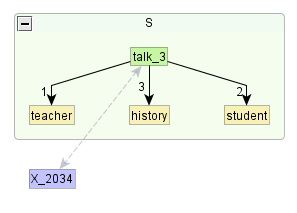
\includegraphics[width=0.4\textwidth, trim = {0cm 0cm 0cm 0cm},clip]{ch6/figs/root.png}
	\caption{Création de la racine à partir du noeud dominant}
	\label{deroulement0}
\end{figure}

\subsection{Sélection du patron de régime dans le lexicon}:
Ensuite, une fois que le noeud dominant est lexicalisé, la règle \emph{actant\_gp\_selection} est déclenchée. Celle-ci permet à GenDR de récupérer les traits encodés dans gp. Puis, à l'intérieur de gp, il y a les traits \texttt{id} et \texttt{dia}. Ces traits sont donc récupérés par la règle et apposé sur le noeud racine. La racine est maintenant contrainte d'utiliser le patron de régime x si la diathèse qu'elle a correspond aux mêmes actants demandés par la structure d'input.

\begin{figure}[htb]
	\centering
	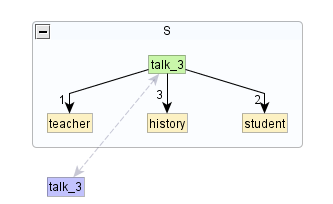
\includegraphics[width=0.4\textwidth, trim = {0cm 0cm 0cm 0cm},clip]{ch6/figs/selectiongp.png}
	\caption{Application de la règle actant\_gp\_selection}
	\label{deroulement1}
\end{figure}

\subsection{Application de la règle actancielle: \emph{actant\_gp\_ijk}}
À l'étape précédente, le noeud \lex{talk\_3} se fait imposer les restrictions suivantes: une paire identifiant de gp et diathèse. Ces traits sont essentiels à l'application des règles actancielles. La règle actant\_gp\_ijk est sélectionnée lorsque la diathèse précise qu'il y a trois actants sémantiques. Il faut aussi que les actants sémantiques que la diathèse précise se retrouve dans la structure sémantique donnée. Sinon, aucune règle actancielle n'est appliquée et la réalisation s'interrompt laissant une racine comme output. 

Ce mécanisme est nouveau puisque dans l'ancienne version de GenDR, le système analysait liaison actancielle individuellement, puis faisait correspondre cet liaison sémantique à une relation syntaxique. Cela se traduisait par la création d'un arc entre la racine et un noeud vide et on y ajoutait des contraintes sur ce noeud simultanément. La version actuelle de GenDR ne fonctionne plus ainsi. Une fois que le gp est sélectionné, on confirme à l'aide du trait dia quel règle actancielle il faudra choisir. Dans notre exemple, ce sera celle-ci puisqu'elle correspond à un gouverneur sélectionnant trois actants.

La règle actant ijk, crée 3 arcs en partance talk\_3 au bout desquels se trouvent des noeuds vides sans contraintes. Elle s'occupe aussi du passage des arcs sémantiques à syntaxique. Le patron de régime qui nous concerne est le suivant: \lstinline!gp = { id=NP_V_PP_about_topic_PP_to_co_agent dia=132 }!. On peut y lire que la diathèse précise que le 1 actant sémantique reste le 1er actant syntaxique, mais que le deuxième actant syntaxique est le 3e sémantique et ainsi de suite. Elle crée donc les arcs syntaxiques à partir de ces informations et ils sont vides.

\begin{figure}[htb]
	\centering
	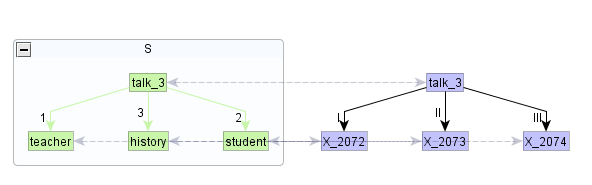
\includegraphics[width=1\textwidth, trim = {0cm 0cm 0cm 0cm},clip]{ch6/figs/actant_gp_ijk.png}
	\caption{Application d'une règle actancielle: actant\_gp\_ijk}
	\label{deroulement2}
\end{figure}

\subsection{Application des contraintes sur les noeuds}
Dans l'ancienne version de GenDR, la règle actancielle contraignait aussi les noeuds nouvellement créés en syntaxe. Notre système a dû créé une règle séparée de la règle actancielle pour des raisons d'efficacité. Nous avons ainsi créé une règle qui contraints chaque noeud nouvellement créé à partir des informations demandées par le patron de régime pour chaque actant syntaxique. Bref, la règle récupère les restrictions sur les noeuds dans le gpcon tel qu'on le voit à la figure \ref{gpexemple}. La règle s'applique donc 3 fois puisqu'il y a trois noeuds vides. On a maintenant trois noeuds contraints.

\subsection{Lexicalisation des noeuds contraints}
Ensuite, on répète une règle de lexicalisation. Dans ce cas il s'agit de \emph{lex\_standard} puisque tous les sémantèmes figurent dans le semanticon et le lexicon. La règle s'applique trois fois car il y a trois noeuds. Puis la lexicalisation réussi à chaque fois puisque ces lexèmes satisfont les contraintes imposées aux noeuds.
\begin{figure}[htb]
	\centering
	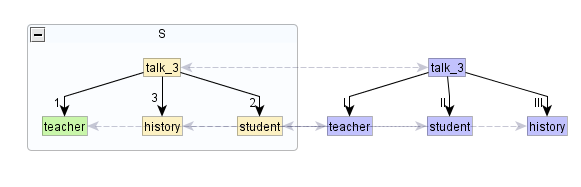
\includegraphics[width=1\textwidth, trim = {0cm 0cm 0cm 0cm},clip]{ch6/figs/lex.png}
	\caption{Applications d'une règle de lexicalisation: lex\_standard}
	\label{deroulement3}
\end{figure}

\subsection{Application de la règle \emph{actant\_gp\_selection}}
Finalement, la règle \emph{actant\_gp\_selection} s'applique encore, mais cette fois-ci pour les lexèmes \lex{teacher},\lex{student} et \lex{history}. Cette règle récupère leurs traits gp.id et gp.dia. Comme ce sont tous des noms communs, ils héritent du gp par défaut de la classe nominale id=NP dia=1 (nous n'avons pas plus d'information sur les patrons de régime des noms compte tenu que VerbNet se spécialisait dans les verbes, mais il existe d'autres ressources parmi celles que nous avions mentionnées qui pourrait combler cette lacune. C'est pourquoi nous n'avons que un gp pour les noms et qu'il est doté d'une diathèse simple permettant de faire la relation complément du nom). encore puisque ces nouveaux noeuds lexicalisés déclenchent l'application de la règle. Dès qu'un x a un gp, on va le repêcher, même si on s'en sert pas après. Si l'un d'entre eux avait eu un complément du nom, alors la sélection du gp aurait prouvé son utilité. C'est une application systématique.

Bref, l'application de toutes ces règles à notre input(figure \ref{input-text}) a permi son arborisation. Nous décrirons dans la section suivante le passage vers la structure syntaxique de surface.

\subsection{Lexicalisation de surface}
La première étape est de lexicaliser en surface les lexèmes profonds. Cette règle récupère aussi la partie du discours de surface de l'entrée lexicale. Le procédé est le même que nous avons vu au chapitre \ref{chapgendr}.

\subsection{Règles actancielles de surface}
Une fois que les lexèmes sont réalisés en surface, les règles actancielles de surface sont déclenchées. Trois règles actancielles de surface seront appliquées puisqu'il y a 3 arcs de dépendances (I, II et III) à réaliser. Concrètement, la règle récupère la valeur du trait \texttt{rel}. 

Donc, la règle synt\_subj est déclenchée et le système récupère l'information sur l'actant syntaxique qui possède le trait texttt{rel}. Comme nous avons choisi l'arborisation à partir du gp \emph{NP\_V\_PP\_to\_co\_agent\_PP\_about\_topic}, le système récupère l'information suivante: \lstinline! I={rel=subjective dpos=N}!. Le produit est le changement d'étiquette de la relation pour la valeur \texttt{subjective}.

Simultanément, la règle \emph{synt\_actant\_prep} est déclenchée une première fois pour faire la correspondance entre l'arc syntaxique qui lie \lex{talk\_3} et \lex{history}. La règle récupère ainsi le code suivant: \lstinline! II={rel=oblique dpos=N prep=about}!. Cela signifie que l'actant syntaxique II correspond à la relation \texttt{oblique} en RSyntS. Cette règle est déclenchée car l'un des actants syntaxiques s'expriment en syntaxe de surface à l'aide d'une préposition (une lexie fonctionnelle). Cela a pour incidence que le noeud où profond de \lex{history} se scinde en deux afin que la préposition \lex{about} face le pont entre le verbe et l'objet indirect qu'il sélectionne. Ce phénomène est illustré par la figure~\ref{deroulement4}. 

Cette règle se déclenche une seconde fois pour traiter l'actant syntaxique III \lex{students}.

\subsection{Règles des déterminants}
Finalement, la règle det\_def réalise les déterminants qui doivent apparaître en syntaxe de surface. Ceux-ci correspondent aux traits que nous avions encodés dans l'input de départ. Seul \lex{teacher} et \lex{student} gouverneront des déterminants puisque leurs représentations sémantiques demandaient que les noeuds soit définis d'une certaine manière en syntaxe de surface. La règle de déterminant réalise \lex{the} lorsque c'est défini et \lex{a} lorsque le noeud est marqué comme indéfini. Il s'agit d'une règle propre à l'anglais.
\begin{figure}[htb]
	\centering
	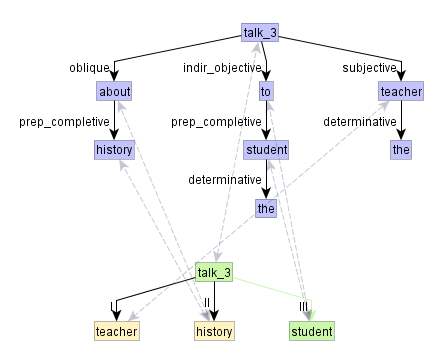
\includegraphics[width=0.5\textwidth, trim = {0cm 0cm 0cm 0cm},clip]{ch6/figs/ssynt.png}
	\caption{Applications des règles actancielles et réalisation des lexies fonctionnelles}
	\label{deroulement4}
\end{figure}
Cela met fin à notre section implémentation. Nous passerons donc à la phase d'évaluation pour vérifier si notre système performe tel que nous l'avions prévu.

\section{Évaluation}
Avant d'entrer dans le vif du sujet, il serait pertinent de faire un bref retour sur les méthodes d'évaluation en \ac{GAT}. \cite{ReiterInvestigationValidityMetrics2009} expliquent qu'il y existe trois types classiques d'évaluation. Ils nomment d'abord la méthode d'évaluation qui se base sur l'exécution d'une tâche en utilisant les textes génénés automatiquement. Ils nomment aussi la méthode d'évaluation humaine. Et finalement, ils parlent des méthodes métriques (automatiques). \cite{ReiterBuildingNaturalLanguage2000} s'étant penché plus tôt sur la question de la validité des méthodes d'évaluation automatiques, ils étaient en faveur d'une évaluation faite par des humains. Toutefois, environ une décennie plus tard, \cite{ReiterInvestigationValidityMetrics2009} remarquaient que les méthodes d'évaluation automatiques se faisaient de plus en plus populaires. Notamment, la méthode BLEU qui avait été développée, à la base, pour les systèmes de traductions automatiques. Nous ferons donc un bref survol de ces méthodes pour décider laquelle se prête le mieux à notre expérience.

BLEU a été créé à la base pour évaluer les rendements des traductions automatiques. Il s'agissait de comparer des outputs d'un système de traduction automatique à un ensemble de traductions humaine (servant de point de référence). Comme la traduction automatique et la génération automatique comportent toutes les deux l'aspect automatique, des chercheurs comme (Langkilde 2002; Habash 2004) ont estimé que la \ac{GAT} bénéficierait de cette méthode d'évaluation. Toutefois, lors de son passage à SemEval2017, FORGe a notamment été évalué par des méthodes métriques et \cite{DBLP:conf/semeval/MilleCBW17} ont fait une brève critique de cette méthode. Ils soulignent que BLEU évalue effectivement bien la couverture, mais comporte des lacunes pour analyser la qualité de chaque output. Leur système avait un score au dessus de la moyenne pour ce qui était de l'évaluation humaine, mais avait reçu un score plus faible pour selon la méthode BLEU. Ils expliquent ce décalage en mentionnant que FORGe mettait de l'avant la qualité de ses outputs par rapport à la quantité. De sorte que ce système filtre à deux reprises les constructions fautives ou potentiellement fautives. (Scoot et Moore, 2007) donnaient aussi quelques mises en garde de la méthode BLEU en précisant qu'elle n'évalue pas toujours correctement des propriétés linguistiques cruciales.

Les méthodes d'évaluation basées sur l'exécution d'une tâche à l'aide de textes générés automatiquement sont assez courantes selon \cite{ReiterInvestigationValidityMetrics2009}. Ces auteurs estiment qu'il s'agit de la méthode qui évalue le mieux le contenu des réalisations d'un système de \ac{GAT}. Toutefois, ils nous mettent en garde que c'est malheureusement la méthode la plus coûteuse en termes de temps et de ressources. En résumé, plus l'output est lisible et clair, plus hautes sont les chances que la tâche soit réalisée rapidement et correctement. Cette méthode n'est pas toujours facile à mettre en place car il faut trouver des participants prêt à donner de leur temps pour lire les rapports générés et effectuer une tâche correspondate. 

Finalement, il y a l'évaluation humaine, plus simple à faire que la méthode à base de tâche, mais plus lente que la méthode automatique. Toutefois, cela reste une méthode très populaire dans le domaine. Il s'agit de coter les outputs en fonction de leur performance à produire des phrases syntaxiquement et sémantiquement acceptables au bon jugement d'un évaluateur.

Considérant ces trois méthodes, nous devons en exclure deux: celle qui est basée sur une tâche et la méthode automatique. D'abord notre système ne réalise pas du texte dans un but précis. On n'a pas de tâche à effectuer pour tester la validité des réalisations. De plus, nous n'avions ni le temps, ni les ressources pour entreprendre ce type d'évaluation. Ensuite, nous ne pouvons pas utiliser la méthode automatique car notre système génère des arbres de dépendances de surface. Les systèmes utilisant la méthode automatique comparent des chaînes de caractères (des réalisations de surface où les textes sont linéarisées et morphologisés). Il nous est donc impossible de comparer nos arbres syntaxiques de surface avec du texte. Il ne reste qu'une méthode d'évaluation s'offrant à nous et c'est celle faite par des humains basée sur nos jugements.

\subsection{Mise en place de l'évaluation}
Pour procéder à l'évaluation de notre système, nous avons utilisé les outputs du script \ref{structurepython} (voir le chapitre \ref{python}). Ceux-ci étaient des structures sémantiques vides dépourvues de prédicats et d'arguments. Il n'y avait que le code pour encadrer le graphe et le texte à reproduire sémantiquement. Nous avons comblé les 978 structures vides en y encodant les unités et relations sémantiques qui correspondaient à l'énoncé. La tâche est simple, nous passerons ces structures sémantiques en input à notre système et nous évaluerons les réalisations produites.

Comme nous avions une quantité limité de temps, nous avons décidé de prendre un échantillon des 978 strucutres sémantiques. Nous en avons choisi 75 aléatoirement. Parmi celles-ci, 25 ont servi à une partie développement précédent la phase d'évaluation comme telle. Ces 25 structures ont été passées au système afin de voir quels sont les problèmes immédiats que nous pouvons réglés sans vérifier si la qualité des arbres produits. Cette phase de développement nous a permi de constater qu'une bon nombre de nos inputs comportaient des problèmes. Nous avons donc noté le type de problème que les inputs comportaient afin de corriger le tir pour la partie évaluation. La partie de développement nous a aussi permi de constater que certains lexèmes appartenant à des PDD différentes apparaissaient en double dans notre dictionnaire. Autrement dit, le verbe \lex{work} et le nom \lex{work} ont la même forme, le système ne sait pas comment les différencier. Cela a donc une incidence sur la réalisation puisque le système construit l'arbre syntaxique à partir du premier lexème qu'il récupère. Donc si nous avions besoin du verbe dans l'arbre et que le système choisi le nom, la réalisation échouera nécessairement. C'est pourquoi nous avons procédé à un filtrage massif de ces cas. Nous les avons réglé en créant une entrée sémantique dans le semanticon qui contiendra les deux entrées lexicales: une version verbale et une version nominale. Elles seront distinguées ainsi dans le semanticon: \lstinline! work { lex = work_n  lex= work_2} !. Bref, nous n'avons pas analysé en profondeur la nature des générations à cette étape, nous voulions seulement répertorier et corriger les problèmes de surface. 

Ensuite, nous avons passé au peigne fin chacun des inputs qui seront évalués. Nous nous sommes assurés que les problèmes d'entrées lexicales répertoriés dans la partie développement étaient corrigés en vue de l'évaluation.

Finalement, nous avons pu procéder à la phase de tests. Nous avons testé les 50 structure sémantiques restantes. Pour ce faire, nous avons développé un script qui générait automatiquement toutes les représentations visuelles et textuelles des passages RSem-RSyntP et RSyntP-RSyntS. La partie visuelle permettait de regarder les différentes constructions d'arbres rapidement pour voir lesquelles étaient des réussites ou des échecs. La partie textuelle nous permettait de voir les informations sur les noeuds. Par exemple, quel était le patron de régime sélectionné pour cette arborisation ou alors, quelle était la diathèse sélectionnée, ou la partie du discours demandée par le noeud, etc. Ces informations ne sont pas explicitées dans le format graphique de présentation des outputs.  

\draft{demander à François comment on devrait calculer la précision. 
Est-ce que la réalisation de 9 arbres grammaticaux pour 1 input est 9/9 ou 1/9 puisqu'il n'y a qu'un arbre qui recrée exactement la phrase qu'on souhaite générer. En choisissant 1/9, on met les réalisations grammaticales et les réalisations incorrectes dans le même bateau. Donc j'ai fait mon évaluation en choisissant 9/9, mais j'ai les chiffres pour l'autre évaluation de la précision. J'ai l'impression que ça rend plus justice au système de considérér que chaque réalisation grammaticale est une victoire du système. Qu'en penses-tu ?}


Nos critères d'évaluation étaient les suivants: le rappel et la précision. Notre évaluation du rappel était binaire. Si l'arbre syntaxique de surface correspondait à la phrase que nous tentions de réaliser, alors la structure recevait la note 1. Dans le cas contraire elle reçoit 0. Pour ce qui est de la précision, nous l'avons évalué comme suit. Pour le nombre d'outputs générés par structure, combien sont des arbres syntaxiquement et sémantiquement corrects représentant la phrase d'input (ou une partie de la phrase). Concrètement, nous avons évalué le rappel ainsi: \[\frac{\text{le nombre de réalisation réussies}}{50}\]. Nous avons ensuite traduit cette fraction en pourcentage. Puis, nous avons noté la précision en la représentant ainsi:\[\frac{\text{le nombre de réalisations grammaticales}}{\text{le nombre de réalisations générées}}\]. Nous avons aussi converti cette fraction en pourcentage.

\draft{demander à François comment on devrait calculer la précision. Est-ce que la réalisation de 9 arbres corrects pour 1 input est 9/9 ou 1/9 ? Parce que si on considère que c'est 1/9, alors on met les mauvaises réalisations et les réalisations grammaticales dans le même bateau.}
\FL{si pour un input tu produis 9 arbres et que ces 9 sont corrects, alors c'est 9/9. P=nb arbres corrects/nb arbres générés}
Nos critères étaient les suivants: le rappel et la précision. Pour notre expérience, le rappel s'évaluait de manière binaire. Si l'arbre syntaxique de surface correspond à la phrase que nous tentons de réaliser, alors la structure reçoit la note 1. Dans le cas contraire elle reçoit 0. Pour ce qui est de la précision, nous l'avons évalué comme suit. Pour le nombre d'outputs générés par structure, combien sont des arbres syntaxiquement et sémantiquement corrects représentant la phrase d'input (ou une partie de la phrase). Concrètement, pour le rappel nous évaluons le nombre total de 1 sur 50 (le nombre de structures testées). Puis, pour la précision, le nombre total de réalisations acceptables représentant la phrase (ou une partie de la phrase) sur le nombre de réalisations générées. Nous devons préciser une partie de la phrase puisque tous les patrons de régime d'une classe s'appliquent tel que nous l'avons vu dans l'exemple. Ainsi, un changement de diathèse donnera une réalistion acceptable, mais pas exactement la phrase qu'on veut représenter, et peut réaliser une partie de l'input sémantique comme dans 'the teacher talked about history' est une réalisation permise par l'input sémantique puisqu'il y a les actants nécessaires dans l'input et un patron permettant de réaliser cette phrase. Nous les avons compté parmi des réussites de précisions, car le but du système est de voir si l'implémentation de VerbNet dans GenDR s'est opérée correctement.
\FL{ta présentation du rappel et de la précision est inutilement compliquée. P=nb str correctes/nb str générées, R=nb str attendues qu'on peut générer/nb str attendues}

En ce qui concerne l'évaluation de la précision, nous avons décidé de considérer comme étant de bons résultats les réalisations paraphrastiques et partiellement représentative de l'input. Cela est une conséquence de la manière que notre système effectue l'arborisation. Comme nous l'avons vu dans l'exemple, le système générait 9 arbres corrects en surface à partir d'un input. Donc, on compterait cela comme une note de \( \frac{9}{9} \). Le but de l'évaluation est aussi de vérifier si l'implémentation de VerbNet dans GenDR génère des phrases grammaticales.
                              
\subsection{Le rappel}

Selon notre évaluation, le taux de rappel se situe à 64\%. Toutefois, ce taux peut monter à 72\% dès qu'on omet quelques erreurs d'encodage qui ont réussi à passer entre les mailles du filet. Ces erreurs d'encodage n'auraient que quelques minutes à corriger. Nous avons répertorié cinq problèmes majeurs qui ont négativement affecté le rappel. Ceux-ci sont de natures diverses: erreurs humaines, erreurs de VerbNet, problème d'incompatibilités théoriques, problème de MATE/GenDR.

Les erreurs humaines répertoriées sont du même type que celles que nous avions remarquées lors de la phase de développement. Nous en avons relevé quatre. L'une des erreurs provenait de l'input et les 3 autres provenaient d'informations erronnées dans les dictionnaires.

Quelques erreurs nous sont directement transmises de VerbNet. Ainsi, il y avait quelques cas où la structure sémantique demandait l'usage d'un prédicat x qui se traduit par un verbe en syntaxe, mais ce verbe était absent de VerbNet. Donc comme ce prédicat liait des actants, l'arborisation de ces relations n'a pas pu se faire puisque GenDR n'avait pas accès aux patrons de régime du prédicat en question. Il y aussi eu quelques cas où la structure sémantique aurait demandé un patron de régime Y de la part du prédicat, mais que ce patron de régime ne figurait pas parmi la liste dans le dictionnaire. Prenons la phrase \form{I want to do it}, si on n'a pas l'entrée de \lex{do}, la réalisation finale sera vouée à l'échec.

Les problèmes suivants sont de nature plus profondes. Parmi les structures qui ont failli au rappel, plusieurs le doivent à un problème d'interface sémantique-syntaxe entre la théorie Sens-Texte et les patrons de régime de VerbNet. Ce que nous voulons dire par là est qu'il y a des cas où la représentation sémantique de la phrase ne cadre aucunement avec les patrons de régime qui s'offre à elle pour réaliser le passage de la sémantique à la syntaxe. Cela fait en sorte que la réalisation de la phrase sera nécessairement un échec. Par exemple, VerbNet considère que la phrase \form{This flyer and that flyer differ} peut se traduire par le patron de régime gp = { id=NP\_V dia=1 }. Toutefois, on se sentirait coupable de plier nos principes théoriques pour faire "fitter" les gp de VerbNet. Donc, nous avons mis en input que differ sélectionnait 2 actants sémantiques. Et nous avons laissé le soin au système de faire échouer cette réalisation. 

De plus, en implémentant les classes verbales dans GenDR, nous avons noté d'autres problème d'interface entre la \ac{TST} et VerbNet. 
x laughed in embarasment 
x slept the sleep of the dead. 

verbe support, collocation :'X took a flight' et qu'on considère que c'est took le verbe, sémantiquemet c'est faux. Take a flight est une collocation, dont le verbe support took n'est là que pour supporté le lexème flight. On pourrait paraphraser par flew. et on ne perdrait pas le sens. Devrait pas être dans le gp de take, mais plutôt dans les propriétés lexicales de flight, qui est sémantiquement fly. 

Finalement, le dernier problème qui a le plus affecté le rappel est la défectuosité du mécanisme d'héritage des gps entre les classes dominées et les classes dominantes. Il s'agit du mécanisme dont nous vantions les mérites au début du chapitre. Concrètement, il s'agit d'un moyen qui fait en sorte qu'une class x pointe vers une classe y et hérite des traits encodés dans la classe y. C'est ainis que nous voulions implémanter l'architecture de VerbNet dans notre système. Mais il se trouve que le mécanisme d'héritage des traits fonctionne partiellement. Tel que présenté dans le début du chapitre, les unités lexicales pointent vers des classes verbales, une classe verbale peut pointer vers une autre classe verbale, et les classe verbales non-dominées pointent vers la classe verbe. Celle-ci donne les traits dpos=V et spos=verb à tous les lexèmes pointant vers des classes verbales. Ce mécanisme d'héritage foncitonne. Effectivement les unités lexicales réalisées ont tous les dpos et spos de la classe verbale, ce qui est un signe que le trait s'est propagé. Mais les patrons de régime ne semblent pas se transmettre d'une classe dominante à une classe dominée. Cela démontre donc que l'héritage des traits est partiel puisque les traits dpos et spos on transcendé toutes les classes subséquentes, mais les traits id et dia qui sont enfouis dans les traits gp (donc deux niveaux de profondeurs) n'ont pas fonctionné. Donc ce problème provient de MATE qui n'est pas capable de transmettre l'héritage d'un trait qui est enfoui dans un trait. Pour pallier à ce problème, on pourrait directement implémanter tous les gps des classes dominantes dans les classes dominées. Ainsi on garde l'architecture pensée de VerbNet où les classes héritent des patrons des autres classes. Le défaut de cette solution est que notre dictionnaire sera saturé d'information. Puisqu'il existe énormément de sous-classe. Cette solution est facilement adaptable puisque nous avons encore les scripts Python ayant servi à extraire les patrons de régime et à créer le lexicon. Nous n'avons qu'à modifier le script pour que chaque sous-classe hérite explicitement des gps des classe qui les domine. Évidemment, cela aura aussi un impact direct sur la précision, puisque dans notre expérience les verbes pointant vers une sous-classe x générait donc les gp de seulement les gp de la sous-classe. Si on fait ça, alors à chaque fois qu'on puise dans une sous-classe, tous les gps hérités feront aussi des tentatives de réalisation, ce qui alourdira le tout. Mais c'était ce qu'on avait prévu au début. Nous n'avions pas vu venir ce problème. Donner un exemple de ce problème. L'input x nécessite l'application du gp y pour la lexie z. La lexie z pointe vers une sous-classe w. Toutefois le gp y se trouve dans la classe mère et le système n'est pas capable d'aller le chercher puisque l'héritage des gps est deffectueux. Donc la réalisation de cet input devient impossile

\subsection{Précision}

En ce qui concerne la précision, nous avons un taux brut de (51\%).\FL{ouf, c'est bas! il faut distinguer entre les structures cul-de-sac et les vrais erreurs. ça te donne combien de P/R sur DEV?} Toutefois, si nous excluons les réalisations qui ne sont que l'application des deux premières règles (root et lex) 58\%. Le fait qu'une réalisation s'arrête brusquement après la racine est en quelque sorte une victoire du système puisque, le système a créé le noeud racine (systématique) puis l'a lexicalisé (systématique) et est aller chercher son gp avec gp selection (systématique) et la réalisation s'est arrêtée puisque le diathèse sélectionnée avec le gp ne correspondait pas aux actants sémantiques demandés par l'input. C'est un peu comme le système de FORGe qui estompe la réalisation lorsqu'il sait que ça me marchera pas. Finalement, en omettant les erreurs humaines d'encodage de notre part, ça nous amène à un taux de précision de 62\%.

\draft{Voici les pourcentages si on considère que la précision s'intreprète comme suit. Le calcul de l'arbre qu'on voulait générer /(sur) toutes les réalisations de surface (comprenant les réalisations grammaticales mais pas extacement correspondantes à l'input). Cela nous donnerait 23\%. Mais si on exclut la réalisation de la racine seule et les erreurs humaines, ça monte à 30\% .}

Ce qui a affecté la précision:
Mis à part la réalisation de la racine seule et des erreurs humaines, voici les phénomènes qui ont affecté la précision.

(si on considère les arbres partiels mais bons comme des erreurs de précision: Cela est dû aux patrons de régime le permettant et à notre module grammatical qui dit au système d'appliquer tous les patrons de régime possibles de la classe si la diathèse le permet. Exactement comme nous avons vu dans l'exemple au début où nous avions 9 réalisations de surface pour 1 input.)

Un cas classique qui est encodé dans plusieurs entrées de patron de régime est le cas où deux prépositions sont listées par VerbNet pour le même actant syntaxique. Par exemple, dans l'évaluation on a vu x. Et la sélection de la préposition y lors de la réalisation de surface rendait la phrase agrammaticale. quand deux prépositions compétitionnent pour le même actant syntaxique, le système génère les 2. C'est un problème qui nous est hérité de VerbNet et que nous n'avions pas prévu puisque nous pensions que VerbNet avait prévu des scénarios où deux prépositions compétitionnent pour la même place, mais qu'ils ne seront jamais parfaitement interchangeables. The doctor cured pat of pneumonia et the docteur cured pat out of pneumonia.

Une bonne partie du noise vient du fait que quand on réalise les gps, tous ceux d'une classe sont réalisés en surface. Le système prend le noeud dominant, il va cherhcher son équivalent dans le lexicon. celui-ci pointe vers une classe. Cette classe a des gps. Puis la règle sélection gp s'applique et pour chaque gp sélectionné, le système crée un nouvel arbre. Seuls ceux qui ont une diathèse qui correspond à la diathèse demandée en input seront réalisés encore plus loin et ceux qui ont un gp qui correspond à la diathèse d'une partie de l'input (teacher talked about history). C'est comme ça que notre système fonctionne et oui, ça créé du noise à chaque fois, mais on pourrait facilement s'en débarassé avec un filtre qui retire les constructions où on a seulement un noeud racine de l'arbre.

Toutefois, ce mécanisme cause du bruit quand un gp est sélectionné parce que les actants sémantiques demandées et ceux fournis par le gp sont un match. Là, il est possible qu'un gp soit utilisé et que ça mène à une réalisation de surface. Toutefois, il peut fort probablement y avoir une incompatibilité sémantique entre l'input et le gp, ce qui fait qu'il sera généré correctement en syntaxe, mais que la phrase est agrammaticale pour des raisons sémantiques ().

Ce mécanisme du à la manière que nos règles sont écrites affecte aussi le bruit en décuplant les arbres lorsqu'une structure d'input possède deux unités sémantiques qui se lexicalisent par des verbes. Effectivement le deuxième verbe pointe vers une classe verbale qui elle encode des patrons de régime, qui seront ensuite sélectionnés par la règle actant gp selection une fois que le noeud du deuxième verbe sera lexicalisé. Cela va donc créer des arbres différents jusqu'à ce que tous les ids des patrons de régime du deuxième verbe seront collés sur le noeud de l'arbre syntaxique profond. Cela génère donc des arbres différents à chaque fois. Exemple :quand on a deux verbes, puisque le système génère une réalisation différente pour chaque gp possible, même si I want to eat: on va avoir tous les gps possible de want , puis pour chaque gp de want permettant la réalisation de eat, on va aussi avoir tous les différents gp de eat qui vont se mettre sur le noeud eat, mais qui n'auront aucun impact sur la syntaxique puisque eat ne prend pas d'argument dans cette construction. Mais les noeuds réalisés sont différents donc ça génère un arbre de plus par gp de eat.

\subsection{Synthèse de l'évaluation}

Ce qu'on retire de tout cela sont deux problèmes majeurs. Le mécanisme d'héritage qui fonctionne partiellement avec l'architecture présente qui nuit au rappel et le mécanisme de sélection de patrons de régime post-lexicalisation qui nuit à la précision. Tel que nous l'avons mentionné, nous pouvons résoudre à court terme le problème d'héritage en implémentant les gps hérités directement dans les sous-classes. Toutefois, la solution à ce problème ne va qu'accentuer le second problème lié à la précision. Effectivement, en réglant le problème de cette façon, on augmente le nombre d'occurrence de l'application de la règle actant gp selection puisqu'elle devra s'appliquer pour tous les gps ajoutés dans la sous-classe.Toutefois, cela impliquerait un dictionnaire bcp plus lourd. Et cela impliquerait encore plus de noise. Ça augmenterait nettement le rappel, mais ça affecterait négativement la précision. À moins qu'on se dote d'un mécanisme pour filtrer les outputs.

De plus, il faut aussi tenir compte du fait que nous avons testé sur 5\% des structures d'input. Mais nous pensons que c'est un 5\% significatif car les problèmes mentionnés sont peu et ils apparaissaient plus d'une fois.

\draft{faire un retour sur l'évaluation en général, amener de nouvelles idées ?}
